% 斜坐标系

\pentry{直角坐标系}

斜坐标系是通常的直角坐标系的延伸.以二维空间中为例,任取两根相互不平行的坐标轴$x$和$y$,都能对平面上任意一点$P$进行定位,方法是认为坐标轴上已经给定了标尺,从$P$处画一条平行于$y$轴的直线,它与$x$轴相交处的标尺数值即为$P$的$x$坐标;类似地,画一条平行于$x$轴的直线,它与$y$轴相交处的标尺数值即为$P$的$y$坐标.

\begin{figure}[ht]
\centering
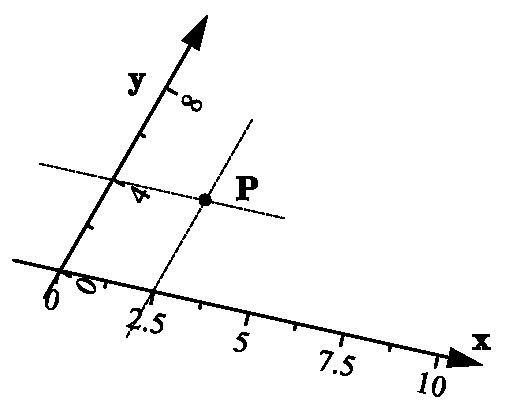
\includegraphics[width=7cm]{./figures/ObSys_1.pdf}
\caption{一个斜坐标系的示意图.图中$x$、$y$两轴的夹角是$72.9^\circ$,两轴的标尺已经给出.在这个坐标系中,$P$的坐标是$<2.5, 4>$.} \label{ObSys_fig1}
\end{figure}

斜坐标系的标尺不一定是均匀的.事实上,只要标尺数值沿着坐标轴的方向一直递增就可以.

\subsection{与直角坐标的转换}

为方便计,我们只考虑标尺均匀的斜坐标系.

给定直角坐标系$xOy$,由相互垂直的$x$轴和$y$轴构成,两轴交于原点$O$.另给定斜坐标系$x'Oy'$,由$x'$轴和$y'$轴构成,两轴在直角坐标系中的斜率分别为$T_x=\tan{\theta_x}$和$T_y=\cot{\theta_y}$,也相交于原点$O$.

\begin{figure}[ht]
\centering
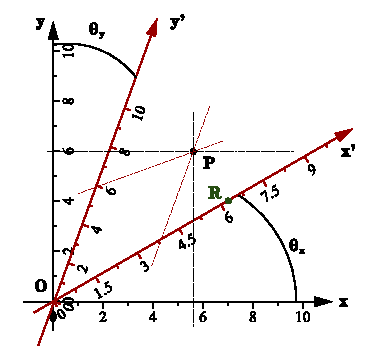
\includegraphics[width=10cm]{./figures/ObSys_2.pdf}
\caption{本小节中所使用的坐标系和点示意图.} \label{ObSys_fig2}
\end{figure}

如果把两个斜坐标轴看成直角坐标轴中的直线,那么我们可以研究斜坐标轴上两点之间的距离.假设取定$x'$轴上一点$R$,在直角坐标系中,$R$到$O$的距离是$|RO|$.如果$x'$轴和$x$轴用相同的标尺,那么$R$在斜坐标系中的坐标应该是$(|RO|, 0)$.但是,如果$x'$轴和$x$轴所用的标尺不一样,那么$R$在斜坐标系中的坐标$(R_{x'},0)$就不再等于$(|RO|, 0)$.这个时候,为了方便描述斜坐标系的标尺,我们引入一个新的概念:\textbf{拉伸比例}.

如果把$x'$轴看成可压缩和伸长的轴线,那么当它被拉伸时,其标尺“密度”会下降,也就是说,$x'$轴上标尺数值为$1$的点到$O$的距离会越来越大.$x'$轴伸长的比例,被称为$x'$轴的\textbf{拉伸比例},大小为$|RO|/R_{x'}$.这样一来,如果$x'$轴的\textbf{拉伸比例}是$r_x$,那么在直角坐标系中$x'$轴上长度为$L$的线段,在斜坐标系中长度就是$L/r_x$.

设有点$P$,其直角坐标为$(x_0, y_0)$,斜坐标为$(x'_0, y_0')$.在直角坐标系中,把两条斜坐标轴和两条平行斜坐标轴而穿过$P$的直线方程写出来,分别联立,可以解出$P$的\textbf{斜坐标投影}的直角坐标,进而得到投影点在直角坐标系中到$O$的长度,将其除以拉伸比例后即可得到相应的$x'$和$y'$坐标.

\begin{example}{斜坐标系的转化}
对于在直角坐标系中的斜率分别为$T_x=\tan{\theta_x}$和$T_y=\cot{\theta_y}$,也相交于原点$O$的斜坐标轴,若$x'$和$y'$的拉伸比例分别为$r_x$和$r_y$,且点$P$的直角坐标为$(x_0, y_0)$,求证$P$的斜坐标为$(x_0', y_0')=(\frac{y_0-T_yx_0}{T_x-T_y}\cdot\frac{\sqrt{1+T_x^2}}{r_x}, \frac{x_0-T_xy_0}{T_y-T_x}\cdot\frac{\sqrt{1+T_y^2}}{r_y})$
\end{example}

\textbf{证明:}

$x'$轴在直角坐标系中的表达式为$y=T_xx$,将它和过$P$且平行于$y'$轴的直线$y=T_yx+y_0-T_yx_0$联立,解得$P$在$x'$轴上投影的位置$(\frac{y_0-T_yx_0}{T_x-T_y}, \frac{y_0-T_yx_0}{T_x-T_y}\cdot T_x)$,其到$O$的距离为$\frac{y_0-T_yx_0}{T_x-T_y}\cdot\sqrt{1+T_x^2}$.考虑到拉伸比例$r_x$,可知$P$在斜坐标系中的$x'$坐标为:$\frac{y_0-T_yx_0}{T_x-T_y}\cdot\sqrt{1+T_x^2}/r_x$.

同理可解得\footnote{也可以利用对称性,将上式中一切$x$和$y$对换得到.}$P$在斜坐标系中的$y'$坐标为:$\frac{x_0-T_xy_0}{T_y-T_x}\cdot\sqrt{1+T_y^2}/r_y$.

\textbf{证毕.}

\subsection{与几何向量的联系}

把直角坐标系中的点$P=(x_0, y_0)$可以看成是从原点$O$指向$P$的向量$\overrightarrow{OP}$.令沿着$x$轴正方向的单位向量为$\mathbb{e_x}$,沿着$y$轴正方向的单位向量为$\mathbb{e_y}$,那么有$\overrightarrow{OP}=x_0\mathbb{e_x}+y_o\mathbb{e_y}$.

从原点出发给定$x'$轴,$y'$轴,以及它们的拉伸比例$r_x$,$r_y$.令沿着$x'$轴正方向的单位向量为$\mathbb{e_{x'}}$,沿着$y'$轴正方向的单位向量为$\mathbb{e_{y'}}$,点$P$在此斜坐标系中的坐标为$(x_0',y_0')$,那么有$\overrightarrow{OP}=x'_0r_x\mathbb{e_{x'}}+y'_or_y\mathbb{e_{y'}}$.

也就是说,斜坐标可以看成是以$r_x\mathbb{e_{x'}}$和$r_y\mathbb{e_{y'}}$作为基底来表达的$\overrightarrow{OP}$的分量.




